\chapter{Magnetic separation configuration}\label{ch:magneticSeparationConfiguration}
%\emph{Simulation software such as ANSYS Maxwell makes it possible to simulate complex magnet geometries, without the need of time consuming and laborious experimental work. This chapter will look at two new magnet geometries which improve the existing magnetic configurations for continuous separation.}

\section{Introduction}\label{sec:introduction}
The primary step was to design a novel magnet configuration that would reduce magnetic particle interaction with the side walls of the microfluidic channel and to enable the continuous separation of magnetic particles of any susceptibility. 

The magnetic field and force were calculated in a 3D geometry for two reference systems, depicted in Figure~\ref{fig:magnetConfigurations}. The two  geometries have two or four magnets, which are placed at the side of a microfluidic channel. The configurations use N42 Neodymium magnets of dimension $20\times 6\times 1.5$ mm (First4Magnets$^\textsuperscript{\textregistered}$,UK), which could be machined and thus, change shape.

\begin{figure}[htb]
\centering
	\begin{subfigure}[b]{0.48\textwidth}
		\includegraphics[width=0.75\textwidth]{img/chapters/magnetDesign/doubleMagnetConfigurationCoordSys.png}
		\caption{}
		\label{fig:double}
    \end{subfigure}
    %%%%%%%%%%%%%%%%
	\begin{subfigure}[b]{0.48\textwidth}
		\includegraphics[width=\textwidth]{img/chapters/magnetDesign/quadrupoleMagnetConfigurationCoordSys.png}
		\caption{}
		\label{fig:quadrupole}
	\end{subfigure}
\caption[3D Schematic of the two magnet configurations]{3D schematic of the two magnet configurations used drawn in ANSYS Maxwell. a) double magnet configuration. b) quadrupole magnet configuration. The dimensions of the magnets are $20\times 6\times 1.5$ mm.}%
\label{fig:magnetConfigurations}
\end{figure}

The numerical simulations were calculated using ANSYS Maxwell. The domain where the simulations were performed was limited by a box, which was simulated as air. The box was chosen to be $100\%$ bigger in all directions than the closest magnetic geometry edge in the corresponding direction. This way it can be ensured that no boundary effects influence the results. 

All numerical results for the magnetic $\mathbf{B}$ field and the magnetophoretic driving force were obtained by using the previously described techniques for FEM and smoothing.  

\subsection{Double magnet configuration}\label{subsec:doubleMagnetConfiguration}
The double magnet configuration shown in Figure~\ref{fig:doubleMagnetConfiguration} is one of the basis geometries here. The two magnets are placed on top of the other in an attractive configuration, with both magnetizations pointing in the same direction. The microfluidic channel will be located along the $x$ axis to the right of the magnet configuration as depicted in Figure~\ref{fig:doubleMagnetConfiguration}. 

\begin{figure}[htb]%
\centering
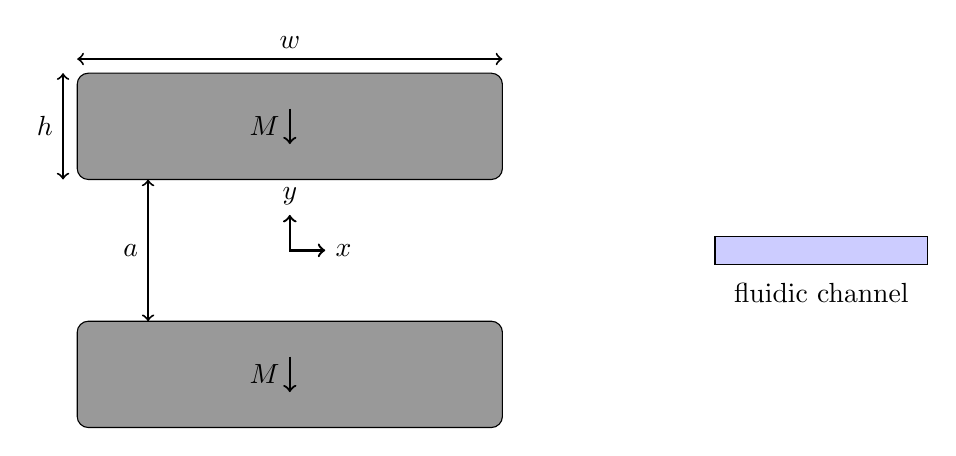
\begin{tikzpicture}[scale=0.9]
	\filldraw[rounded corners, fill=black!40!white, draw=black] (-9,1) rectangle (-3,2.5);
	\filldraw[rounded corners, fill=black!40!white, draw=black] (-9,-1) rectangle (-3,-2.5);	
	\filldraw[fill=blue!20!white, draw=black] (0,-0.2) rectangle (3,0.2);	
	\node[thick] at (1.5,-0.6) {fluidic channel};
					
	\draw[line width=0.3mm,<->] (-6,0.5) node[anchor=south] {$y$} -- (-6,0) -- (-5.5,0) node[anchor=west] {$x$};

	\draw[thick,->] (-6,2) -- node[thick,anchor=east]{$M$} (-6,1.5);
	\draw[thick,->] (-6,-1.5) -- node[thick,anchor=east]{$M$} (-6,-2);
	\draw[line width=0.25mm,<->] (-9,2.7) -- node[anchor=south]{$w$} (-3,2.7);
	\draw[line width=0.25mm,<->] (-9.2,1) -- node[anchor=east]{$h$} (-9.2,2.5);
	\draw[line width=0.25mm,<->] (-8,-1) -- node[anchor=east]{$a$} (-8,1);
\end{tikzpicture}
\caption[2D diagram of the double magnet configuration]{2D slice diagram ($z=0$) of the double magnet configuration used to generate the external magnetic field for separation. The rectangular permanent magnets (grey) are set up in attraction, with the magnetization in the negative $y$ direction as indicated by the magnetization vector $M$. The parameter $w$, $h$ and $a$ describe the with, the height and the separation of the two magnets. The microfluidic channel is located (light blue) to the right of the dipole configuration. The schematic is not drawn to scale.}%
\label{fig:doubleMagnetConfiguration}%
\end{figure}

The three geometric parameters of the system, notified in Figure~\ref{fig:doubleMagnetConfiguration}, and their ratios are used to quantify the distribution of the magnetic field and force; height $h$ and width $w$ of the magnets and their vertical spacing $a$. Two different ratios are studied here: $h/w$ (aspect ratio) and $w/a$ (relative gap). The magnetic force calculation and its smoothing are performed at the post processing level.

As a conservative field ($\mathbf{\nabla} \cdot \mathbf{B} = 0$), an essential property of the magnetic flux density is the formation of complete closed flux loops around the magnet. The loops' spatial distribution is a function of the number, position and magnetization orientation of the magnets, as shown in Figure~\ref{fig:magneticFluxDensityDoubleMagnetConfiguration}, which represents the vector field of the magnetic flux density $\mathbf{B}$. In the double magnet configuration, they go straight from one magnet towards the other, forming a big loop around the two magnets. This is the case in the middle of the magnets, while near the edge the lines enlarge and finally tend to form a loop around only one magnet. This configuration shows an interesting characteristic in the horizontal centre plane ($y=0$) and its vicinity (see Figure~\ref{fig:doubleMagnetConfiguraitonMagneticDrivingForce}). 

\begin{figure}[htb]
   \centering
   \includegraphics[width=0.7\textwidth]{img/chapters/magnetDesign/doubleMagnetConfiguration_bField_inclMagnet.eps}
   \caption[Simulated vector field of the magnetic flux of the double magnet configuration]{Vector representation of the magnetic flux density $\mathbf{B}$ at $z=0$. The grey rectangles represent the magnet cross-section.}
   \label{fig:magneticFluxDensityDoubleMagnetConfiguration}
\end{figure}

Magnetic particles will be stationary in a magnetic field if either the magnitude of the flux density is zero ($|\mathbf{B}|=0$) or there is no field gradient ($\nabla|\mathbf{B}|=0$). Figure~\ref{fig:doubleMagnetConfiguraitonMagneticDrivingForce} shows the exerted forces on a single magnetic particle along the $x$-axis at a slice where $z=0$. Areas where the magnetic particles are attracted (A) towards the magnets and areas where particles are getting repulsed (R) from the magnet alternate. The fact that attractive and repulsive forces are alternating also means that there are regions where the particles experience no driving force. However, these points are not always a stable gathering point and their position depends on the magnet configuration geometry parameters. 

\begin{figure}[htb]%
\centering
   \includegraphics[width=0.7\textwidth]{img/chapters/magnetDesign/doubleMagnetConfigurationMagneticForce.png}
\caption[Magnetic force on a single magnetic particle along the $x$ axis when exposed to the magnetic field of the double magnet configuration]{Magnetic force on a single magnetic particle of $1$ $\mu$m in diameter in the $x$ direction. The particle is assumed to have the magnetic properties of Chemicell particles. The letters A and R indicate the region where the particle experiences an attractive or a repulsive force, respectively. The shaded area (grey), depicts the edge of the magnet configuration.}%
\label{fig:doubleMagnetConfiguraitonMagneticDrivingForce}%
\end{figure}

%%%%%%%%%%%%%%%%%%%%%%%%%%%%%
%The advantage of using a magnetic field of this design is the minimising of the number of MPs at the edges of the MFD, where the velocity profile is zero. Due to the zero magnetic force acting on the MPs in the ROE, theoretically, MPs of any susceptibility, size and concentration can be separated from a sample flow. % Naomi

\subsubsection{Effects of magnet aspect ratio}\label{subsubsec:effectsOfMagnetAspectRatio}
Figure~\ref{fig:doubleMagnetConfigurationMagneticDrivingForceAndFluxDensityForDifferentAspectRatio} shows the  magnetic flux density distribution and its magnetophoretic driving force on the $x$ symmetry axis, for different aspect ratios $h/w$ ranging from $0.1$ to $3$. In the reported case, the magnet width $w$ and vertical separation of the magnets $a$ are kept constant at $6$ mm and $2$ mm, respectively, while its height is varied. Only one half of the system is considered in these results because the flux density is symmetric about the $y$ axis. Since the magnetic flux density is plotted along the $x$ axis only the $y$ component of the $\mathbf{B}$ field is plotted, which will be referred to as $B_{y}$.

\begin{figure}[!htb]
\centering
	\begin{subfigure}[b]{0.48\textwidth}
		\includegraphics[width=\textwidth]{img/chapters/magnetDesign/doubleMagnetConfigurationMagneticFluxDensityForDifferentAspectRatio.eps}
	\caption{}
    \label{fig:doubleMagnetConfigurationMagneticFluxDensityAspectRatio}
    \end{subfigure}
    \hfill
	\begin{subfigure}[b]{0.48\textwidth}
		\includegraphics[width=\textwidth]{img/chapters/magnetDesign/doubleMagnetConfigurationMagneticDrivingForceForDifferentAspectRatio.PNG}
	\caption{}
	\label{fig:doubleMagnetConfigurationMagneticDrivingFroceAspectRatio}
	\end{subfigure}
\caption[Magnetic $B$ field of the double magnet configuration and its magnetophoretic driving force along the $x$ symmetry axis for different magnet aspect ratio]{Magnetophoretic driving force of the double magnet configuration and its corresponding magnetic $B$ field along the $x$ symmetry axis for different aspect ratio $h/w$ ranging from $0.1$ to $3$. (a) Magnetic flux density. (b) Magnetophoretic driving force. The dashed blue line indicates the magnet edges of the double magnet configuration.}%
\label{fig:doubleMagnetConfigurationMagneticDrivingForceAndFluxDensityForDifferentAspectRatio}
\end{figure}

Two stable gathering points for magnetic beads in solution can be identified from Figure~\ref{fig:doubleMagnetConfigurationMagneticDrivingFroceAspectRatio}. One in the middle of the dipole configuration ($x=0$) and one that is outside of the dipole configuration ($x>3$ mm). These stable gathering points are important for the trapping and manipulation of the magnetic beads because any small disturbance to the particles' position will result in a restorative force to return them to the same point. There also exists an unstable gathering point that is associated with the point in which $B_{y} = 0$, caused by the change in flux direction between the inner and outer faces of the magnets. In this region particles move away from this position if they are not spot on and thus should be avoided when conducting experiments. 

The first of the stable gathering points ($x=y=z=0$), is actually a stable equilibrium point and has already been investigated by Gassner et al.~\cite{Gassner2009}. Figure~\ref{fig:doubleMagnetConfigurationMagneticDrivingForceAndFluxDensityForDifferentAspectRatio} suggests that higher aspect ratios (i.e. bar magnets) are suitable for magnetic particle isolation in this first case. This is attributable to the increase in both the magnitude and gradient of $B_{y}$ for $|x| < 3$ mm, and therefore an increase in the magnitude and gradient of magnetophoretic driving force at higher aspect ratios. However, this is not the case for the gathering point of interest that lies outside the dipole configuration. In fact, it is shown in Figure~\ref{fig:doubleMagnetConfigurationMagneticDrivingFroceAspectRatio} that the increase in aspect ratio has little effect on increasing the magnetophoretic driving force around the maxima, and at higher aspect ratios (e.g. $h/w = 3$) can even lead to a significant decrease of the magnetophoretic driving force as the gathering point position is pushed further away from the magnets where the magnetic field is weaker. The gradient of the flux density is also smaller around the maxima (shallower peak in $B_{y}$) and so there is a lower magnetophoretic driving force around the equilibrium as shown in the inset of Figure~\ref{fig:doubleMagnetConfigurationMagneticDrivingFroceAspectRatio}.

An increase in aspect ratio does not affect the position of the stable equilibrium within the dipole ($x=y=z=0$), but pushes the stable gathering point outside of the dipole further away from the double magnet configuration. The position of the latter stable equilibrium appears to have a linear relationship with the aspect ratio, as shown in Figure~\ref{fig:stableGatheringPointAspectRatio}.

\begin{figure}[!htb]%
\centering
	\includegraphics[width=0.7\textwidth]{img/chapters/magnetDesign/doubleMagnetConfigurationGatheringPointAspectRatio.eps}
\caption[Behaviour of position of the static gathering point as a function of the magnet aspect ratio]{Behaviour of the position of the static gathering point at the outside of the double magnet configuration as a function of the magnet aspect ratio $h/w$.}
\label{fig:stableGatheringPointAspectRatio}%
\end{figure}

\subsubsection{Effects of vertical separation between magnets}\label{subsubsec:EffectsOfVerticalSeparationBetweenMgnets}
Figure~\ref{fig:doubleMagnetConfigurationMagneticDrivingForceAndFluxDensityForDifferentSeparationRatio} shows the evolution of the $\mathbf{B}$ field as well as the resulting magnetophoretic driving force as a function of the relative gap $a/w$. The aspect ratio $h/w$ of the magnet is kept constant at $0.25$ ($w=6$ mm and $h=1.5$ mm) and only the spacing $a$ is varied.

\begin{figure}[!htb]
\centering
	\begin{subfigure}[b]{0.48\textwidth}
		\includegraphics[width=\textwidth]{img/chapters/magnetDesign/doubleMagnetConfigurationFluxDensityForDifferentSeparationRatio.eps}
	\caption{}
    \label{fig:doubleMagnetConfigurationMagneticFluxDensitySeparationRatio}
    \end{subfigure}
    \hfill
	\begin{subfigure}[b]{0.48\textwidth}
		\includegraphics[width=\textwidth]{img/chapters/magnetDesign/doubleMagnetConfigurationMagneticDrivingForceSeparationRatio.PNG}
	\caption{}
	\label{fig:doubleMagnetConfigurationMagneticDrivingFroceSeparationRatio} %%%%%
	\end{subfigure}
\caption[Magnetic $B$ field of the double magnet configuration and its magnetophoretic driving force along the $x$ symmetry axis for different separation ratio]{Magnetophoretic driving force of the double magnet configuration and its corresponding magnetic $B$ field along the $x$ symmetry axis for different separation ratios $a/w$ ranging from $0.2$ to $1$. (a) Magnetic flux density. (b) Magnetophoretic driving force. The dashed blue line indicates the magnet edges of the double magnet configuration.}%
\label{fig:doubleMagnetConfigurationMagneticDrivingForceAndFluxDensityForDifferentSeparationRatio}
\end{figure}

Increasing the relative gap results in both a lower magnitude of $B_{y}$ and gradient around the peak as shown in Figure~\ref{fig:doubleMagnetConfigurationMagneticFluxDensitySeparationRatio}. This in turn leads to a lower magnitude and gradient of the magnetophoretic driving force in and around the particle gathering region outside of the magnet configuration (see Figure~\ref{fig:doubleMagnetConfigurationMagneticDrivingFroceSeparationRatio}) and thus the \textit{separation power} will be decreased.

Plotting the position against the relative gap $a/w$, in Figure~\ref{fig:stableGatheringPointSeparationRatio}, shows again an apparent linear relationship between $a/w$ and the stable gathering position outside of the magnet configuration.

\begin{figure}[!htb]%
\centering
	\includegraphics[width=0.7\textwidth]{img/chapters/magnetDesign/doubleMagnetConfigurationGatheringPointSeparationRatio.eps}
\caption[Behaviour of position of the static gathering point as a function of the magnet separation ratio]{Behaviour of position of the static gathering point outside of the magnet configuration as a function of magnet separation ratio $a/w$.}
\label{fig:stableGatheringPointSeparationRatio}
\end{figure}

There is an obvious limit to this geometry which is a relative separation of $a/w=0$, where no gathering point outside of the geometry will occur. However, this extreme boundary is not the only limiting factor. The stable gathering points will also vanish if the horizontal centre line ($x$ axis) is vertically moved closer to the top or the bottom magnet. Therefore, the microfluidic channel must be positioned on the centre plane between the two magnets ($y=0$) in order to minimise vertical forces. Due to this constraint and the manufacturing process of the iBidi fluid channels, a minimum vertical separation $a_{min}$ of only $2.64$ mm can be achieved. 

\subsubsection{Effects of tapered magnets}\label{subsubsec:effectsOfTaperedMagnets}
As seen previously, changing the thickness or the vertical spacing of the magnets, alters strength of the magnetophoretic driving force as well as the position of the static gathering points. By tapering the magnets, these two effects can be combined. Tapering the magnets was also considered as a method of gradually reducing the magnetophoretic driving force in order to gently release particles into the flow at the tail-end of the magnets.

The two magnet shapes that incorporate a taper are shown in Figure~\ref{fig:taperedMagnetSchematic}, where the taper is either on the inner faces (Figure~\ref{fig:taperInner}) or the outer faces (Figure~\ref{fig:taperOuter}), beginning halfway along the length of the magnets and growing in the $z$ direction. In these diagrams, the channel will flow from left to right whilst the magnetic force on the particles mainly acts in the $x$ and $y$ direction. The tapers are modelled using N42 Neodymium magnets of dimension $20\times 6\times 1.5$ mm, with the magnets getting progressively thinner until it is half the non-tapered thickness at the end and the vertical separation is set to $a=2.6$ mm.  

\begin{figure}[htb]
\centering
	\begin{subfigure}[b]{0.48\textwidth}
	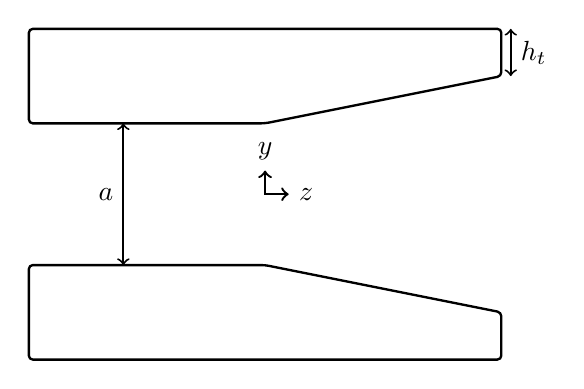
\begin{tikzpicture}[scale=0.6]
		\draw [line width=0.3mm, rounded corners=0.5mm] (0,1.5)--(-5,1.5)--(-5,3.5)--(5,3.5)--(5,2.5)-- cycle;	
		\draw [line width=0.3mm, rounded corners=0.5mm] (0,-1.5)--(-5,-1.5)--(-5,-3.5)--(5,-3.5)--(5,-2.5)-- cycle;			
		\draw[line width=0.3mm,<->] (0,0.5) node[anchor=south] {$y$} -- (0,0) -- (0.5,0) node[anchor=west] {$z$};
	\draw[line width=0.25mm,<->] (-3,-1.5) -- node[anchor=east]{$a$} (-3,1.5);
	\draw[line width=0.25mm,<->] (5.2,2.5) -- node[anchor=west]{$h_{t}$} (5.2,3.5);
	\end{tikzpicture}
	\caption{}
    \label{fig:taperInner}
    %%%%%%%%%%%%%%%%%%%%%%%%
    \end{subfigure}
    \hfill
	\begin{subfigure}[b]{0.48\textwidth}
	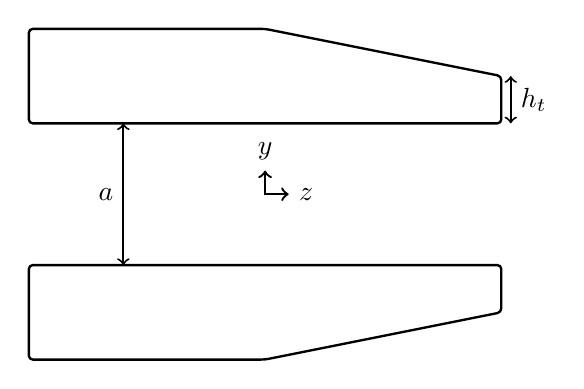
\begin{tikzpicture}[scale=0.6]
		\draw [line width=0.3mm, rounded corners=0.5mm] (-5,1.5)--(-5,3.5)--(0,3.5)--(5,2.5)--(5,1.5) -- cycle;	
		\draw [line width=0.3mm, rounded corners=0.5mm] (-5,-1.5)--(-5,-3.5)--(0,-3.5)--(5,-2.5)--(5,-1.5) -- cycle;	
		\draw[line width=0.3mm,<->] (0,0.5) node[anchor=south] {$y$} -- (0,0) -- (0.5,0) node[anchor=west] {$z$};
	\draw[line width=0.25mm,<->] (-3,-1.5) -- node[anchor=east]{$a$} (-3,1.5);	
	\draw[line width=0.25mm,<->] (5.2,1.5) -- node[anchor=west]{$h_{t}$} (5.2,2.5);	
	\end{tikzpicture}
	\caption{}
	\label{fig:taperOuter}
	\end{subfigure}
\caption[Diagrams of the tapered magnet configurations]{Diagrams of the tapered magnet configurations: a) inner taper b) outer taper. The taper begins halfway along the length of the magnets and finishes at half the non-tapered thickness of the magnets. Schematic is not drawn to scale.}%
\label{fig:taperedMagnetSchematic}
\end{figure}

From Figure~\ref{fig:taperedMagnetDrivingForce} it can be concluded that for both taper configurations, the larger the taper (i.e. the thinner the magnet), the lower the magnetophoretic driving force and its gradient around the static gathering point, although the effect is more pronounced for the magnets which are tapered on the inner faces. This is due to the fact that the vertical magnet separation increases with this taper configuration. The particle gathering positions are also affected by the size of the taper, either pushing the gathering points out for magnets with inner tapers or pulling the gathering points in for magnets with outer tapers (see inset Figure~\ref{fig:taperedMagnetDrivingForce}).

\begin{figure}[!htb]
\centering
	\begin{subfigure}[b]{0.48\textwidth}
		\includegraphics[width=\textwidth]{img/chapters/magnetDesign/innerTapering.PNG}
	\caption{}
    \label{fig:innterTaperDrivingForce}
    \end{subfigure}
    \hfill
	\begin{subfigure}[b]{0.48\textwidth}
		\includegraphics[width=\textwidth]{img/chapters/magnetDesign/outerTapering.PNG}
	\caption{}
	\label{fig:outerTaperDrivingForce} 
	\end{subfigure}
\caption[Approximations of the behaviour of magnetophoretic driving force for different values of tapered thickness]{Approximations of the behaviour of magnetophoretic driving force for different values of tapered thickness: a) inner taper b) outer taper. Conditions are for magnets with dimensions $w=6$ mm and $h=1.5$ mm at a separation of $a=2$ mm. The values are taken along the $x$ symmetry axis. Tapered thickness: $d_{t}=1.5$ mm, $d_{t}=1.25$ mm, $d_{t}=1.0$ mm and $d_{t}=0.75$ mm. The edge of the magnets is shown as the vertical dotted line.}%
\label{fig:taperedMagnetDrivingForce}
\end{figure}


\subsection{Quadrupole magnet configuration}\label{subsec:quadrupoleMagnetConfiguration}
By adding a second double magnet configuration the double magnet configuration geometry can be extended to a quadrupole configuration, where the microfluidc channel is assumed to be always in the centre of the geometry. A 2D schematic of the quadrupole magnet configuration used is shown in Figure~\ref{fig:quadrupoleMagnetConfiguration}.

\begin{figure}[!htb]%
\centering
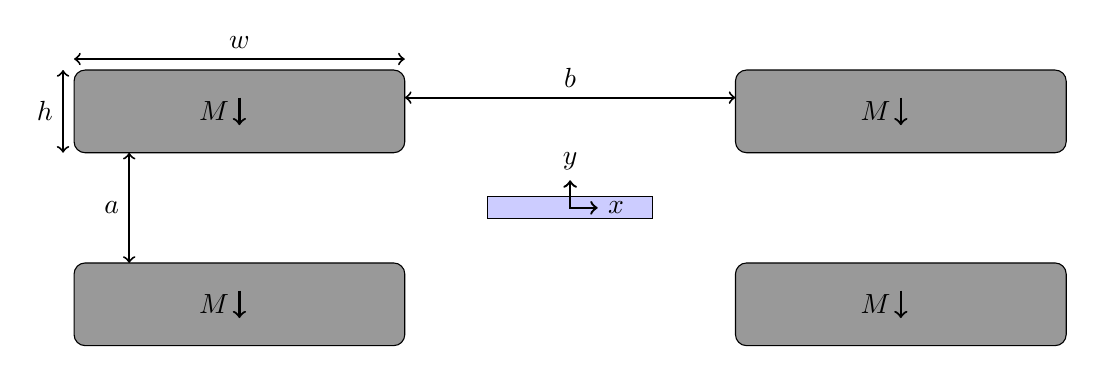
\begin{tikzpicture}[scale=0.7]
	\filldraw[rounded corners, fill=black!40!white, draw=black] (-9,1) rectangle (-3,2.5);
	\filldraw[rounded corners, fill=black!40!white, draw=black] (-9,-1) rectangle (-3,-2.5);	
	\draw[thick,->] (-6,2.0) -- node[thick,anchor=east]{$M$} (-6,1.5);
	\draw[thick,->] (-6,-1.5) -- node[thick,anchor=east]{$M$} (-6,-2.0);

	\filldraw[fill=blue!20!white, draw=black] (-1.5,-0.2) rectangle (1.5,0.2);					
	\filldraw[rounded corners, fill=black!40!white, draw=black] (9,1) rectangle (3,2.5);
	\filldraw[rounded corners, fill=black!40!white, draw=black] (9,-1) rectangle (3,-2.5);	
	\draw[thick,->] (6,2.0) -- node[thick,anchor=east]{$M$} (6,1.5);
	\draw[thick,->] (6,-1.5) -- node[thick,anchor=east]{$M$} (6,-2.0);
	
	\draw[line width=0.3mm,<->] (0,0.5) node[anchor=south] {$y$} -- (0,0) -- (0.5,0)
	 node[anchor=west] {$x$};
	 
	\draw[line width=0.25mm,<->] (-9,2.7) -- node[anchor=south]{$w$} (-3,2.7);
	\draw[line width=0.25mm,<->] (-9.2,1) -- node[anchor=east]{$h$} (-9.2,2.5);
	\draw[line width=0.25mm,<->] (-8,-1) -- node[anchor=east]{$a$} (-8,1);
	\draw[line width=0.25mm,<->] (-3,2) -- node[anchor=south]{$b$} (3,2);
\end{tikzpicture}
\caption[2D diagram of the quadrupole magnet configuration]{2D slice diagram ($z=0$) of the quadrupole magnet configuration used to generate the external magnetic field for separation. The rectangular permanent magnets (grey) are set up in attraction, with their magnetization in the negative $y$ direction. The microfluidic channel is located (light blue) in the centre of the two double magnet configurations. The parameter $w$, $h$, $a$ and $b$ describe the with, the height, vertical separation and horizontal separation of the magnets as indicated in the picture. The schematic is not drawn to scale.}%
\label{fig:quadrupoleMagnetConfiguration}
\end{figure}

The advantage of this configuration compared to the double magnetic configuration is that the magnetophoretic driving force acting on single magnetic particles is increased and that the gathering points (where no horizontal force acts on the particles) will be on the centre plane ($x=0$) for most geometry parameters as will be explained in this section. This leads to a potential increase in particle throughput due to the increased force and because the particles are introduced through both sheath flow channels. However, these advantages come with a price, such that the vertical force on the particle will be higher too, which might cause the particles to migrate to the top and bottom more quickly where they potentially get stuck. Thus, one needs to work out the optimal spacing between the two \textit{sandwich configuration}. 

\subsubsection{Effects of horizontal separation between magnet pairs}\label{subsubsec:EffectsOfHorizontalSeparatinBetweenMagnetPairs}
The magnetic quadrupole configuration is subject to the same geometric characteristics and limitations like the double magnet configuration. Figure~\ref{fig:quadrupoleMagnetConfigurationMagneticDrivingForceForDifferentRatio} shows the magnetophoretic mobility along the $x$ axis for the same aspect ratios $h/w$ and relative gap ratios $a/w$ already used in the double magnet configuration analysis. 

\begin{figure}[!htb]
\centering
	\begin{subfigure}[b]{0.48\textwidth}
		\includegraphics[width=\textwidth]{img/chapters/magnetDesign/quadrupoleMagnetConfigurationMagneticDrivingForceForDifferentAspectRatio.eps}
	\caption{}
    \label{fig:quadrupoleMagnetConfigurationMagneticDrivingFroceAspectRatio}
    \end{subfigure}
    \hfill
	\begin{subfigure}[b]{0.48\textwidth}
		\includegraphics[width=\textwidth]{img/chapters/magnetDesign/quadrupoleMagnetConfigurationMagneticDrivingForceForDifferentSeparationRatio.eps}
	\caption{}
	\label{fig:quadrupoleMagnetConfigurationMagneticDrivingFroceSeparationRatio} %
	\end{subfigure}
\caption[Magnetic driving force of the quadrupole magnet configuration for different aspect and relative gap ratios]{The magnetic driving force along the $x$ axis for different aspect and relative gap ratios. (a) Aspect ratio $h/w$ ranging from $0.1-3$. (b) Relative gap ratio $a/w$ ranging from $0.2-1.0$. The dashed blue lines indicate the edges of the iBidi $\mu$-slide.}%
\label{fig:quadrupoleMagnetConfigurationMagneticDrivingForceForDifferentRatio}
\end{figure}

It can be seen that small ($h/w=0.1$) as well as large ($h/w=3$) aspect ratios negatively effect the horizontal magnetophoretic driving force, because either the magnetic $\mathbf{B}$ field and its gradient becomes very weak or the stable gathering point eventually becomes an unstable one, where a magnetic particle located outside of the coordinate system's origin gets attracted either side (see Figure~\ref{fig:quadrupoleMagnetConfigurationMagneticDrivingFroceAspectRatio}). Similarly, an increasing relative gap ($a/w$) weakens the magnetic flux density and its gradient and thus, lowers the magnetophoretic driving force. Furthermore, the unstable gathering points are pushed towards the centre of the geometry and eventually ($a/w \geq 1$) overlap the stable gathering point (see Figure~\ref{fig:quadrupoleMagnetConfigurationMagneticDrivingFroceSeparationRatio}).

However, besides these two ratios, the magnetic quadrupole configuration also introduces the nondimensional distance ratio $b/a$ (see Figure~\ref{fig:quadrupoleMagnetConfiguration}), which will also be considered here. For this reason, the magnetophoretic driving force has been calculated in the area of the fluid channel ($x = -1.5-1.5$ mm and $y = -0.2-0.2$ mm) for different distance ratios $b/a$. Thereby, the vertical separation $a$ was kept at $2$ mm and only the horizontal distance $b$ between the two double magnet configuration was changed. Figure~\ref{fig:magnetophoreticDrivingForceField} shows the magnetophoretic driving force field of the magnetic quadrupole configurations at $z=0$ for distance ratios $b/a$ ranging from $1.5$ to $3$. 

\begin{figure}[htb]
\centering
	\begin{subfigure}[b]{0.48\textwidth}
		\includegraphics[width=\textwidth]{img/chapters/magnetDesign/quadrupoleMagnetConfigurationMagnetophoreticDrivingForceField_3mmSeparation.eps}
	\caption{$b/a = 1.5$}
    \label{fig:magnetophoreticDrivingForceField_3mm}
    \end{subfigure}
    \hfill
	\begin{subfigure}[b]{0.48\textwidth}
		\includegraphics[width=\textwidth]{img/chapters/magnetDesign/quadrupoleMagnetConfigurationMagnetophoreticDrivingForceField_4mmSeparation.eps}
	\caption{$b/a = 2$}
	\label{fig:magnetophoreticDrivingForceField_4mm}
	\end{subfigure}
	\hfill
	\begin{subfigure}[b]{0.48\textwidth}
		\includegraphics[width=\textwidth]{img/chapters/magnetDesign/quadrupoleMagnetConfigurationMagnetophoreticDrivingForceField_5mmSeparation.eps}
	\caption{$b/a = 2.5$}
	\label{fig:magnetophoreticDrivingForceField_5mm}
	\end{subfigure}
	\hfill
	\begin{subfigure}[b]{0.48\textwidth}
		\includegraphics[width=\textwidth]{img/chapters/magnetDesign/quadrupoleMagnetConfigurationMagnetophoreticDrivingForceField_6mmSeparation.eps}
	\caption{$b/a = 3$}
	\label{fig:magnetophoreticDrivingForceField_6mm}
	\end{subfigure}
\caption[Vector field of the magnetic driving force of the quadrupole magnet configuration across the iBidi $\mu$-slide]{2D magnetic driving force vector field across the iBidi $\mu$-slide cross-section at $z=0$. The vertical gap $a$ is kept constant at 2 mm and only the horizontal distance $b$ is varied from $3-6$ mm. (a) $b/a=1.5$. (b) $b/a=2$. (a) $b/a=2.5$. (a) $b/a=3$}%
\label{fig:magnetophoreticDrivingForceField}
\end{figure}

Due to the width of the iBidi channel ($w_{f}=3$ mm) there is a lower limit on horizontal distance $b$ besides the obvious limit where $b=0$ mm. For distance $b \leq 3$ mm the magnet edges closest to the microfluidic channel will overlap with the channel and therefore cause an always attractive force in their proximity. This will cause magnetic particles not only to move towards the stable gathering point in the centre of the geometry, but also let them migrate towards the magnets, which is an undesirable effect. This is why, the analysis starts at $b=3$.  

In Figure~\ref{fig:magnetophoreticDrivingForceField} it can be seen that the magnetophoretic driving force in $x$ direction gets smaller with an increasing distance ratio, however, also the unwanted vertical driving force is decreased at the same time. This phenomena is again depicted in Figure~\ref{fig:quadrupoleMagnetConfigurationMagneticDrivingForceForDistanceRatio} which shows the horizontal and vertical magnetic driving force along the top edge of the fluid channel ($y=0.2$ mm), which represents the worst case because that is where the vertical force within the channel cross-section is highest. This \textit{worst case} analysis is again done for different distance ratios.

\begin{figure}[htb]
\centering
	\begin{subfigure}[b]{0.48\textwidth}
		\includegraphics[width=\textwidth]{img/chapters/magnetDesign/quadrupoleMagnetConfigurationMagneticDrivingForceForDifferentDistanceRatioHorizontal.eps}
	\caption{}
    \label{fig:quadrupoleMagnetConfigurationMagneticDrivingForceForDistanceRatio_horizontal}
    \end{subfigure}
    \hfill
	\begin{subfigure}[b]{0.48\textwidth}
		\includegraphics[width=\textwidth]{img/chapters/magnetDesign/quadrupoleMagnetConfigurationMagneticDrivingForceForDifferentDistanceRatioVertical.eps}
	\caption{}
	\label{fig:quadrupoleMagnetConfigurationMagneticDrivingForceForDistanceRatio_vertical}
	\end{subfigure}
\caption[Magnetophoretic driving force in horizontal and vertical direction along the top of the iBidi $\mu$-slide]{Magnetophoretic driving force in horizontal and vertical direction along the top of the $\mu$-slide ($y=0.2$ mm) for different distance ratios. (a) Horizontal magnetophoretic driving force. (b) Vertical magnetophoretic driving force.}%
\label{fig:quadrupoleMagnetConfigurationMagneticDrivingForceForDistanceRatio}
\end{figure}

There is a clear trade-off between the horizontal and vertical driving force. However, in order to find the optimum for the horizontal gap between the magnets the ratio of the two components is taken. This ratio is then integrated and tried to be maximised in order to gain the optimal horizontal to vertical magnetic driving force. The figure of merit is depicted in Figure~\ref{fig:optimalHorizontalDistance}. It can be seen that the function has a maximum at $b=4.5$ mm which will be taken as an optimal horizontal magnet distance $b$. Luckily, this optimal value does not conflict with the physical limitations of the iBidi channel, because the minimum separation $a$ is $2.64$ mm, which pushes the unstable gathering points closer to the centre of the geometry. In order to account for that and to ensure the unstable gathering points are kept outside of the channel's cross-section, the horizontal distance $b$ needs to be at least $3.2$ mm.  

\begin{figure}[!htb]%
\centering
	\includegraphics[width=0.7\textwidth]{img/chapters/magnetDesign/optimalHorizontalDistance.eps}
\caption[Accumulated magnetophoretic driving force ratio for different horizontal distances]{This figure shows the integrated value of the absolute ratio between the horizontal magnetic driving force, $S_{x}$, and vertical magnetic driving force, $S_{y}$ along the top edge of the fluid channel ($y=0.2$ mm and $z=0$) for multiple horizontal distances $b$.}
\label{fig:optimalHorizontalDistance}
\end{figure}

\section{Double magnet configuration experiment}\label{sec:doubleMagnetConfigurationExperiment}
The setup shown in Figure~\ref{fig:doubleMagnetConfigurationExperimentSetup} was used to verify the existence of the static gathering points outside of the double magnet configuration for different vertical gaps. A stereo microscope is used because the lower magnification gave a better visualisation of the overall structure of how the particles agglomerate around the gathering point. 

\begin{figure}[htb]%
\centering
	\includegraphics[width=0.8\textwidth]{img/chapters/magnetDesign/doubleMagnetConfigurationExperimentSetup.png}
\caption[Experimental setup to verify static gathering points]{Experimental setup to verify the gathering points of the double magnet configuration for different relative gap ratios $a/w$. Magnets and fluid channel (iBidi $\mu$-slide) are mounted onto L-brackets which can be accurately adjusted using positioning stages. The magnet configuration is shown in more detail in Figure~\ref{fig:doubleMagnetConfigurationExperimentSetupSchematic}.}
\label{fig:doubleMagnetConfigurationExperimentSetup}
\end{figure}

Figure~\ref{fig:doubleMagnetConfigurationExperimentSetupSchematic} shows a schematic of the experimental double magnet configuration setup. The permanent magnets and the fluid channel (iBidi $\mu$-slide) are attached to L-brackets using Araldite$^\text{\textregistered}$ adhesive. The L-brackets are mounted onto translation stages, which allowed accurate control of the vertical gap and height of the double magnets configuration, as well as precise positioning of the iBidi $\mu$-slide. Non-magnetic materials are used wherever possible to minimise the distortion of the magnetic field; the L-brackets are fabricated from aluminium and the fasteners are brass.

\begin{figure}[htb]%
\centering
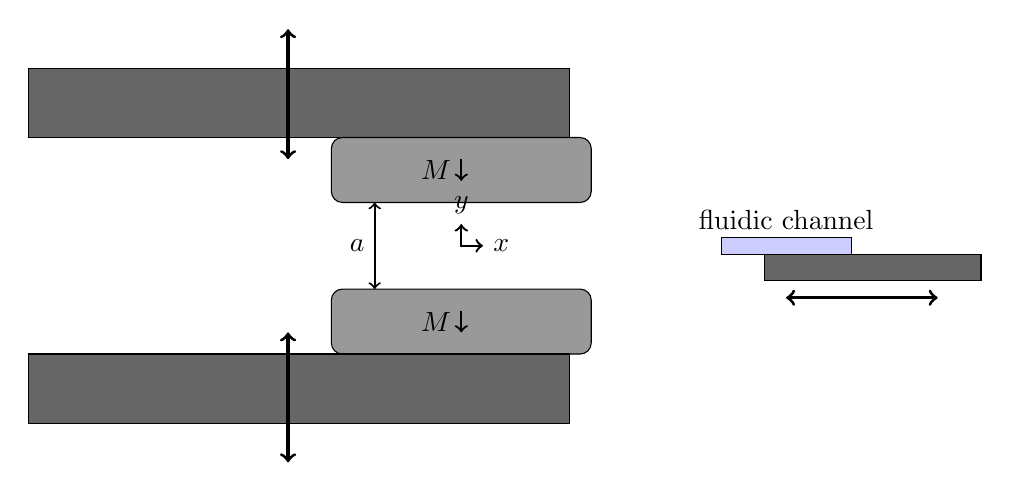
\begin{tikzpicture}[scale=0.55]
	\filldraw[fill=black!60!white, draw=black] (-16,2.5) rectangle (-3.5,4.1);	
	\filldraw[rounded corners, fill=black!40!white, draw=black] (-9,1) rectangle (-3,2.5);
	\filldraw[rounded corners, fill=black!40!white, draw=black] (-9,-1) rectangle (-3,-2.5);
	\filldraw[fill=black!60!white, draw=black] (-16,-2.5) rectangle (-3.5,-4.1);	

	\node[thick] at (1.5,0.6) {fluidic channel};	
	\filldraw[fill=blue!20!white, draw=black] (0,-0.2) rectangle (3,0.2);	
	\filldraw[fill=black!60!white, draw=black] (1,-0.2) rectangle (6,-0.8);	
	\draw[line width=0.4mm,<->] (1.5,-1.2) -- (5,-1.2);

					
	\draw[line width=0.3mm,<->] (-6,0.5) node[anchor=south] {$y$} -- (-6,0) -- (-5.5,0) node[anchor=west] {$x$};

	\draw[thick,->] (-6,2) -- node[thick,anchor=east]{$M$} (-6,1.5);
	\draw[thick,->] (-6,-1.5) -- node[thick,anchor=east]{$M$} (-6,-2);
	\draw[line width=0.25mm,<->] (-8,-1) -- node[anchor=east]{$a$} (-8,1);
	\draw[line width=0.4mm,<->] (-10,2) -- (-10,5);
	\draw[line width=0.4mm,<->] (-10,-2) -- (-10,-5);
\end{tikzpicture}
\caption[Schematic of experimental double magnet configuration setup]{Schematic of experimental double magnet configuration setup, showing the magnets (light grey) and channel (light blue) attached to L-brackets (dark grey). The supporting structure (L-brackets) are mounted onto high precision transverse translation stages to accurately adjust magnet and fluid channel position. The degrees of freedom of the L-brackets are shown by the arrows. Schematic is not drawn to scale.}%
\label{fig:doubleMagnetConfigurationExperimentSetupSchematic}%
\end{figure}

The iBidi $\mu$-slide was filled with particle solution, while the channel was positioned away from the magnets so that the particles within the channel did not have any significant interaction with the magnetic field. The fluid channel was then slowly moved towards the magnets using the horizontal positioning stage. Once in position, the setup was left until the particles have reached their final gathering points and no further observable growth in particle agglomeration formation could be seen. The particles form an elongated and narrow elliptical band of high particle concentration with ends that taper into streams of reducing concentration, as shown in Figure~\ref{fig:doubleMagnetConfigurationParticleFormation}.

\begin{figure}[htb]%
\centering
	\includegraphics[width=0.7\textwidth]{img/chapters/magnetDesign/doubleMagnetConfigurationParticleFormation.PNG}
\caption[Particle formation around gathering points]{Particle formation around gathering points of the double magnet configuration.}
\label{fig:doubleMagnetConfigurationParticleFormation}
\end{figure}

After an equilibrium was reached the gathering position was measured as being the distance from the major axis of the elliptical band to the edge of the magnets, as a best approximation.

The experiment was repeated by pumping a fresh fully dispersed particle solution into the channel and altering the vertical gap. The vertical separation, $a$, was increased in $0.2$ mm intervals from $2.6$ mm to $5.8$ mm, which is equivalent to a relative gap ratio, $a/w$, of $0.44$ to $0.97$. The experiments affirmed the linear relationship between the position of the static gathering points and the vertical separation between the two permanent magnets, which could also be seen in the numerical simulations, as depicted in Figure~\ref{fig:doubleMagnetConfigurationGatheringPointSeparationRatioExperiment}. There is a good quantitative agreement between the experiments and the finite element analysis. Since the magnets move more out of focus for larger relative gap ratios ($a/w$) it becomes more difficult to accurately measure the distance between the magnet edge and the particle band. This effect negatively affects the measurement and explains the negative trend of the data points. 

\begin{figure}[htb]%
\centering
	\includegraphics[width=0.7\textwidth]{img/chapters/magnetDesign/doubleMagnetConfigurationGatheringPointSeparationRatioExperiment.eps}
\caption[Experimentally found position of the gathering points for the double magnet configuration]{Variation of gathering positions with magnet separation for a double magnet configuration using two $20 \times 6 \times 1.5$ mm N42 NdFeB magnets. The experimental results are in good agreement with the linear relationship predicted by the FEA.}
\label{fig:doubleMagnetConfigurationGatheringPointSeparationRatioExperiment}
\end{figure}

\subsection{Tapered double magnet configuration experiment}
The magnets for this experiment were tapered by polishing two $20 \times 6 \times 1.5$ mm N42 NdFeB magnets so that they had the shape shown in Figure~\ref{fig:taperInner}. The thickness of the magnet at the end of the taper was approximately half the non-tapered thickness ($h_{t}=0.75$ mm). There is a clear difference in the static gathering position between the non-tapered half (Figure~\ref{fig:nonTaperedMagnetExperiement}) and the tapered half (Figure~\ref{fig:taperedMagnetExperiement}) of the magnet faces. An observable linear increase in the equilibrium position as the magnets become thinner, as well as a reduction in the bead concentration, is illustrated in Figure~\ref{fig:taperedMagnetExperiement}.

\begin{figure}[!htb]
\centering
	\begin{subfigure}[b]{0.48\textwidth}
		\includegraphics[width=\textwidth]{img/chapters/magnetDesign/doubleMagnetConfigurationGatheringPointPositionExperiment.png}
	\caption{}
    \label{fig:nonTaperedMagnetExperiement}
    \end{subfigure}
    \hfill
	\begin{subfigure}[b]{0.48\textwidth}
		\includegraphics[width=\textwidth]{img/chapters/magnetDesign/doubleMagnetConfigurationGatheringPointPositionExperimentTapered.png}
	\caption{}
	\label{fig:taperedMagnetExperiement}
	\end{subfigure}
\caption[Static particle gathering band for tapered double magnet configuration]{Static particle gathering band for the double magnet configuration using two tapered $20 \times 6 \times 1.5$ mm N42 NdFeB magnets. a) Particle band along the non-tapered edge. b) Particle band along the tapered edge. There is a linear increase in the static equilibrium position with increasing magnet taper.}%
\label{fig:taperedMagnetGatheringPointExperiment}
\end{figure}

\section{Conclusion}\label{sec:conclusionMagneticSeparationDesign}
Two new magnetic separation geometries have been presented and analysed. Both configurations have the unique property that there are regions where no magnetic force acts on a magnetized particle. However, some of these regions are unstable, which means that a small deviation from this region makes the particle migrate somewhere else. 

However, not all of these regions happen to be unstable. There are stable gathering points where particle do not experience a force. These stable regions can be advantageous for magnetic particle separation because any type of magnetic particle will migrate towards these gathering points.

It could be seen that the geometry parameters of the magnetic configurations determine the position of the gathering regions. Due to the thickness of the iBidi $\mu$-slide, the vertical separation $a$ of the magnets is limited to a minimum of $a_{min} = 2.64$ mm. The magnets used (N42 NdFeB) have an aspect ratio of $0.25$. Under these circumstances, the gathering points are horizontally $2.2$ mm away from the magnet edges of the double magnet configuration. For the quadrupole the gathering points lie on the centre plane between the two double magnet configurations. The optimal horizontal distance between the two double magnet configurations was found to be $4.5$ mm due to the balance of the horizontal and vertical force.

The aspect ratio simulations suggest that flat magnets with low aspect ratios will have a stronger separating power than bar magnets with high aspect ratios. Considering that the work in this project is towards the design and fabrication of a compact microfluidic device, this was encouraging because bar magnets would have resulted in bulky devices. The relative separation simulations were important in providing a straightforward method for manipulating the position of the isolated particles simply by increasing or decreasing the vertical separation between them. This can lead to a device capable of adjusting the particle trajectories during continuous flow. Likewise, the simulations of the tapered magnets show the possibility of altering the particle trajectories in a continuous manner. Additionally, the reduction in the magnetophoretic driving force as the taper increases can be useful for releasing the separated particles back into the free-flow of the stream.

The existence of the position of stable, static gathering points outside of the double magnet configuration for different relative gap ratios is also experimentally confirmed. The experimental results closely match the predictions obtained by the numerical simulations. However, the formation of an elliptical particle band made it difficult to precisely determine the position of the static gathering region. The elliptical formation can be explained by the fact that the length of the magnets is not large enough compared to the other geometric parameters of the configuration. Consequently, the end effects of the magnets create a magnetic field gradient in the $z$ direction which cannot be neglected. There is a maxima along the line $z=0$, explaining why the band is the widest at this position and narrows towards the ends of the magnets. Theoretically, the beads should form a thin line along the equilibrium. This is because any finite force equates to the particles having a finite velocity according to the equilibrium between the magnetic force and Stokes drag. The formation of an elliptical band may therefore be explained by other forces that were not previously taken into account.

For the tapered magnets, the linear increase in the position of static equilibrium conforms to the results of the numerical simulation. The reduced concentration of particles towards the end of the taper, where the magnets are thinnest, supports the theory that the gradient of the magnetophoretic driving force is lower compared to the non-tapered section.